\section{Actor Model}
\subsection{A universal modular actor formalism for artificial intelligence}
\bibentry{Hewitt1973}
\subsubsection*{Summary}
``This paper proposes a modular ACTOR architecture and definitional method for artificial intelligence that is conceptually based on a single kind of object'' (p. 235). This position paper is one of the earliest works on the actor model.
\subsubsection*{Notes}
\begin{itemize}
\item The exact details of the paper are less important than the overarching themes, given that actor theory evolved from the time of publication.
\item ``We use the ACTOR metaphor to emphasize the \underline{inseparability of control and data flow}'' (p. 235).
\item ``Every actor has an INTENTION which checks that the prequisites and the context of the actor being sent the message are satisfied. The intention is the \underline{CONTRACT} that the actor has with the outside world'' (p. 235).
\item Some apects of actor-based message passing:
	\begin{itemize}
	\item ``Sending messages between actors is a \underline{universal control primitive} in the sense that control operations{\ldots}are special cases'' (p. 240).
	\item ``Sending a message to an actor makes no presupposition that the actor sent the message will ever send back a message to the continuation'' (p. 241).
	\end{itemize}
\end{itemize}

\subsection{Viewing control structures as patterns of passing messages}
\bibentry{Hewitt1977a}
\subsubsection*{Summary}
Abstract: ``The purpose of this paper is to discuss some organizational aspects of programs using the actor model of computation. In thispaper wepresent an approach to modelling intelligence in terms of a society of communicating knowledge-basedproblem.solving experts. In turn each of the experts can be viewed as a society that can befurther decomposed in the same way until the primitive actors of the system are reached. We are investigating the nature of the communication mechanisms neededfor effective problem-solving by a society of experts and the conventions of civilized discourse that make thispossible. In this way we hope eventually to develop aframework adequatefor the discussion of the central issues o f problem-solving involving parallel versus serial processing and centralization versus decentralization of control and information storage. This paper demonstrates how actor message passing can be used to understand control structures as patterns of passing messages in serial processing.This paper is a prerequisite,for successors which treat issues of parallelism and communication witlzin the framework established here. The ability to analyze or synthesize any kind of control structure as a pattern of passing messages among the members of a societyprovides an important toolfor understanding control structures. Ultimately, we hope to be able to characterize various control structures in common use by societies in terms of patterns of passing messages.''
\subsubsection*{Notes}
\begin{itemize}
\item Demonstrates iteration and recursion as patterns of message passing in the actor model, with event diagrams.
\item As with \cite{Hewitt1973}, the language is very flowery; the utility of this paper is in the high-level concepts that are briefly mentioned.
\item This paper still positions actors as agents in distributed AI.
\item ``We are developing methods to specify the behavior of actors (objects) in terms that are natural to the semantics of the causal and incidental relationships among the objects. That is, we are attempting to develop a \emph{transparent medium} for constructing models in which the control structure emerges \emph{as a pattern of passing messages among the objects being modeled}. Towards that end, we are developing a programming methodology consisting of the following activities:
	\begin{itemize}
	\item \emph{Deciding on the natural kinds of actors (objects) to have in the system to be constructed.}
	\item \emph{Deciding for each kind of actor what kind of messages it should receive.}
	\item \emph{Deciding for each kind of actor what it should do when it receives each kind of message.}`` (p. 325)
	\end{itemize}
\item ``Actors are a local model of computation. There is no such thing as ``action at a distance'' nor is there any ``global state'' of all actors in the universe. Actors interact on a purely local way by sending messages to one another'' (p. 325).
\item ``The basic construct of our computation model is the ACTOR. The BEHAVIOR of each actor is DEFINED by the relationships among the events which are caused by the actor. At a more superficial and imprecise level, each actor may be thought of as having two aspects which together realize the behavior which it manifests:
	\begin{itemize}
	\item the ACTION it should take when it is sent a message;
	\item its ACQUAINTANCES which is the finite collection of actors that it directly KNOWS ABOUT.'' (p. 325--326)
	\end{itemize}
\item ``Note that the KNOWS ABOUT relationship is asymmetric; i.e. it is possible for an actor A to know about another actor C without C also knowing about A. Should it happen that A and B know about each other then we will say that they are MUTUAL ACQUAINTANCES'' (p. 326).
\item ``\emph{The reader should keep in mind that within the actor model of computation there is no way to decompose an actor into its parts. An actor is defined by its behavior; not by its physical representation!}'' (p. 327)
\end{itemize}

\subsection{Laws for communicating parallel processes}
\bibentry{Hewitt1977b}
\subsubsection*{Summary}
Abstract: ``This paper presents some laws that must be satisfied by computations involving communicating parallel processes. The laws are stated in the context of \emph{actor theory}, a model for distributed parallel computation, and take the form of stating plausible restrictions on the histories of parallel computations to make them phyiscally realizble{\ldots}Since the causal relations among the events in a parallel computation do not specify a total order on events, the actor model generalizes the notion of computation from a \emph{sequence of states} to a \emph{partial order of events}.
\subsubsection*{Notes}
\begin{itemize}
\item ``In this paper, we argue that in a distributed computation, the notions of \emph{local state}, \emph{local time}, and \emph{local name space}, should replace those of global state, global time, and global name space'' (p. 2).
\item ``In the actor model, we generalize the notion of computation from that of a sequence of global states [assumed by the serial model of computation] to that of a partial order of events in the system, where each event is the transition from one local state to another'' (p. 2).
\item \textbf{This work could be useful for formally proving correctness of concurrent risk propagation.}
\item ``Computations in the actor model are partial order of events. Hence, specifications for an actor and correctness assertions for a computation can be given very naturally in terms of events and causal relations among events. Since inference rules can use these partial orders directly, the number of cases in proofs is considerably reduced. Thus, actor theory attacks the problem of distributed system design by offering an abstract conceptual and formal model for thinking about and proving theorems about distributed systems'' (p. 1).
\item See below regarding actor orderings, actor induction, and locality.
\end{itemize}
 \includepdf[pages={4-10}]{Hewitt1977b.pdf}

\subsection{Foundations of actor semantics}
\bibentry{Clinger1981}
\subsubsection*{Summary}
Abstract: ``This thesis extends and unifies their [Carl Hewitt's, Irene Greif's, Henry Baker's, and Giuseppe Attardi's] work through the following observations. The ordering laws postulated by Hewitt and Baker can be proved using a notion of global time. The most general ordering laws are in fact equivalent to an axiom of realizbability in globla time. Independence results suggest that some notion of global time is essential to any model of concurrent computation{\ldots}The locality laws postulated by Hewitt and Baker may be proved for the semantics of an actor-based language. Altering the semantics slightly can falsify the locality laws. The locality laws thus constrain what counts as an actor semantics.'' This work also develops a power domain for ``providing a fixed point semantics for a class of nondeterministic programming languages in which a fair merge can be written.''
\subsubsection*{Notes}
\paragraph{General remarks}
\begin{itemize}
\item The power domain, semantics, event diagrams, and proof details are not relevant for my thesis. The following sections are potentially relavant to my thesis for proving correctness or properties of risk propagation.
	\begin{itemize}
	\item Extensions of the ordering laws (p. 16) and locality laws (p. 123) \cite{Hewitt1977b}
	\item Actor semantics (pp. 87--89)
	\end{itemize}
\item Prioritize this work over \cite{Hewitt1977b} when possible.
\end{itemize}

\paragraph{Actor model description}
\begin{itemize}
\item ``Each communication is described as a \emph{message} arriving at a computational agent called an \emph{actor}'' (p. 17).
\item ``The actor model refers to the arrival of a message at an actor as an \emph{event}. Thus all events in the model are arrival events, and there is no such thing as a sending event'' (p. 17).
\item ``The actor that receives a message in an event is called the \emph{target} of the event. The message that the target receives is just called athe message of the event'' (p. 18).
\item ``An event may activate several subseqent events. That is, the arrival of a message at an actor may cause that actor to send outa number of messages to other actors. The events that a given event activates are said to have that event as their \emph{activator}'' (p. 18).
\item An ``\emph{external event}'' is ``an event with no activator (p.  18).
\item ``Chains of activations define the \emph{activation ordering} (p. 19).
\item Indirect dependency may not be expressed by the activation ordering alone (p. 19). The \emph{arrival ordering} ``represents the order in which events occur at a particular target actor. Thus an arrival ordering represents the \emph{local time} of an actor'' (p. 20). The \emph{combined ordering} can address the shortcoming of the activation ordering (p. 19).
\end{itemize}

\paragraph{Ordering laws}
\begin{itemize}
\item The notion of global time is used ``to motivate and improve upon the \emph{ordering laws}'' \cite{Hewitt1977b} (p. 21). The strongest of the three ordering laws form a necessary and sufficient condition for orderings that are realizable in global time (p. 23).
\item \emph{Strong Axiom of Realizability}: there exists a one-to-one mapping $g$ from the events $E$ into the nonnegative reals that preserves the combined ordering $\rightarrow$ and such that $g^{-1}(I)$ is finite for every bounded interval $I \subset \mathbb{R}$. Equivalently, there exists a one-to-one mapping $g: E \rightarrow \mathbb{N}$ that preserves $\rightarrow$ (p. 28).
\item \emph{Weak Axiom of Realizability}: there exists a one-to-one mapping $g$ from the events $E$ into the real numbers $\mathbb{R}$ that preserves the combined ordering $\rightarrow$ and such that $G^{-1}(I)$ is finite for every bounded interval $I \subset \mathbb{R}$. Equivalently, there exists a one-to-one mapping $g: E \rightarrow \mathbb{Z}$ that preserves $\rightarrow$ (p. 29).
	\begin{itemize}
	\item Allows for properties of actor systems to be proven that do not depend upon the existence of some initial state (p. 29).
	\end{itemize}
\item Assuming the Strong Axiom of Realizability...
	\begin{itemize}
	\item ``Most logics that have been proposed for reasoning about parallel programs are based upon sequences of global states. The realizability axioms suggest that the actor model may be made compatible with these logics by treating an event as a change of global state, so that a global time specifies a sequence of global states'' (pp. 31--32). \emph{Realizability axiom connects Asynchronous Convergence Theorem with the actor model to prove convergence properties.}
	\item \emph{Law of Strict Causality} (LSC): for no event $e \in E$ does $e \rightarrow e$ (i.e., $e$ precedes itself) (p. 32).
	\item \emph{Law of Countability} (LC): there are at most countably many events. That is, $E$ is countable, where a finite set is considered countable (p. 32).
	\item \emph{Law of Finite Predeccesion} (LFP): for all events $e'$, the set
		\begin{equation*}
			\{e \mid e \rightarrow e'\}
		\end{equation*}
	is finite (p. 32).
	\item \emph{Theorem}: the Strong Axiom of Realizability is equivalent to the conjunction of LSC, LC, and LFP (p. 32).
	\item Corollaries of LFP (p. 34):
		\begin{itemize}
		\item \emph{Law of Finite Predecession in the Activation Ordering}: for all events $e'$, the set
			\begin{equation*}
				\{e \mid e \overset{act}{\longrightarrow} e'\}
			\end{equation*}
		is finite.
		\item \emph{Law of Finite Predecession in the Arrival Ordering}: for all events $e'$, the set
			\begin{equation*}
				\{e \mid e \overset{arr_a}{\longrightarrow} e'\}
			\end{equation*}
		is finite for a given actor $a \in A$.
		\item
		\end{itemize}
	\end{itemize}
\item Assuming the Weak Axiom of Realizability...
	\begin{itemize}
	\item \emph{Law of Discreteness} (LD): for all events $e_1, e_2$, the set
		\begin{equation*}
			\{e \mid e_1 \rightarrow e \rightarrow e_2\}
		\end{equation*}
	is finite (p. 37).
	\item \emph{Law of Finite Chains Between Events in the Combined Ordering} (LFCBECD): there are no infinite chains of events between two events in the combined ordering $\rightarrow$ (p. 37).
	\item \emph{Theorem}: assume the LSC. Then the LD is equivalent to the LFCBECD.
	\item \emph{Theorem}: the Weak Axiom of Realizability is equivalent to the conjunction of the LSC, the LC, and the LD.
	\item Consequences of the LD:
		\begin{itemize}
		\item \emph{Law of Discreteness in the Activation Ordering}: if $C$ is a chain of events in the activation ordering from $e_1$ to $e_2$, then $C$ is finite.
		\item \emph{Law of Discreteness in the Arrival Ordering}: for all events $e_1, e_2$ such that $T(e_1) = T(e_2) = a$, then
			\begin{equation*}
			\{e \mid e_1 \overset{arr_a}{\longrightarrow} e \overset{arr_a}{\longrightarrow} e_2\}
			\end{equation*}
		is finite.
		\end{itemize}
	\end{itemize}
\end{itemize}

\paragraph{Actor semantics}
\begin{itemize}
\item ``A \emph{primitive serializer}{\ldots}consists of an arbiter, a queue, and a processor. A primitive serializer is the target of an event when a message \emph{arrives} at the serializer's arbiter and is placed in the serializer's queue to await processing. When two messages arrive at about the same time, the arbiter decides which one goes first in the queue. The arbiter must be reliable and place every incoming message in the queue. In other words, the arbiter performs a fair merge on incoming messages. The processor of the primitive serializer \emph{accepts} messages serially from the queue and processes them according to some deterministic and terminating algorithm. When the processor accepts a message from the queue, it \emph{locks} and accepts no more messages from the queue until it finishes with that message.

Messages are accepted and processed in the same order that they arrive at the primitive serializer, that is, in the same order as the arrival ordering of their corresponding events. Processing a message may involve (1) changing the \emph{local state} of the primitive serializer's processor; (2) sending out a finite set of messages; (3) creating a finite set of new primitive serializers; this last possibility resembles process creation. When the processor finishes processing a message, it \emph{unlocks} and accepts the next message in the queue. If there are none, it waits until there are'' (pp. 88--89).
	\begin{itemize}
	\item \emph{The concept of a serializer was first proposed in \cite{Atkinson1977} as an improvement over the concept of a monitor, but Clinger provides a description that more clearly aligns with Akka and how actors are implemented.}
	\end{itemize}
\end{itemize}

\paragraph{Locality laws}
\begin{itemize}
\item ``An actor consists of a \emph{script} and a \emph{vector of acquaintances}. The script is simply the code for the actor{\ldots}The vector of acquiantances may contain pointers to other actors. While the pointers themselves cannot be side effected, the behaviors of the actors pointed to can change when those actors process messages sent to them{\ldots}An actor's vector of acquaintances may contain values other than pointers to other actors, or it may consist solely of pointers. In either case[,] the actors that it points to are called \emph{acquaintances} of the actor. An actor may alter its vector of acquaintances while processing a message, so its set of acquaintances may change over time'' (p. 124).
\item ``The participants in an event are those actors that the target of the event knows about while processing themessage of the event. The participants are thus the acquaintances of the target together with the actors mentioned by the message \cite{Hewitt1977b} (p. 129).
\item \emph{Law of Finite Acquaintances}: $\mathit{acq}(e)$ is finite for every event $e \in E$ (p. 129).
\item \emph{Existence of Participants Function}: there exists a function participants $E \rightarrow \mathit{subsets}(A)$ satisfying the following laws.
	\begin{itemize}
	\item \emph{Finite Interaction Law}: $\mathit{participants}(e)$ is finite for every $e \in E$.
	\item \emph{Original Acquaintances Law}: let
		\begin{equation*}
			\mathit{created}(e) = \{a \in A - A_0 \mid \mathit{creation(a) = e}\}.
		\end{equation*}
	If $a$ is a created actor, that is, $a \in A_0$, and $e$ is the first event in the arrival ordering of $a$, then
		\begin{equation*}
			\mathit{acq}(e) \subseteq \mathit{participants(\mathit{creation(a)}) \bigcup \mathit{created}(\mathit{creation}(a))}
		\end{equation*}
	\item \emph{Arrival Precursor Acquaintances Law}: if $a = T(e)$ and $e$ has an immediate predecessor $e'$ in the arrival ordering of $a$, that is,
		\begin{equation*}
			e' \overset{arr_a}{\longrightarrow} e
		\end{equation*}
	and
		\begin{equation*}
			\lnot \exists e'' [e' \overset{arr_a}{\longrightarrow} e'' \overset{arr_a}{\longrightarrow} e]
		\end{equation*}
	then
		\begin{equation*}
			\mathit{acq}(e) \subseteq \mathit{participants(e') \bigcup \mathit{created}(e')}
		\end{equation*}
	\item \emph{Arrival Acquaintances Law}: if $e \in E$ is not external, then let $\mathit{activator}(e)$ be the activator of $e$, that is, the unique immediate predecessor of $e$ in the activation ordering $\overset{act}{\rightarrow}$. If $e \in E$ is not external, then
		\begin{align*}
			T(e) &\in \mathit{participants}(\mathit{activator}(e)) \bigcup \mathit{created}(\mathit{activator}(e)) \\[10pt]
			\mathit{participants}(e) &\subseteq \mathit{acq}(e) \bigcup \mathit{participants}(\mathit{activator}(e)) \bigcup \mathit{creator}(\mathit{activator}(e)),
		\end{align*}
	\end{itemize}
\end{itemize}

\subsection{Actors: A model of concurrent computation in distributed systems}
\bibentry{Agha1985}
\subsubsection*{Summary}
Contributions (pp. 6--7):
	\begin{itemize}
	\item ``A critical overview of the various proposed models of concurrency.
	\item A simple outline of the actor model and the specification of minimal primitive constructs for actor languages.
	\item A transition system for actor systems and a structured operational semantics for an actor language.
	\item A paradigm for addressing problems in distributed computing which is suitable for computation in open systems.
	\item A model to support compositionality and abstraction from irrelevant detail.''
	\end{itemize}

\subsubsection*{Notes}
\paragraph{General remarks}
\begin{itemize}
\item This work marks a distinct shift toward framing the actor model as a paradigm for concurrent, distributed computing.
\item The description that this work provides on the actor model is much clearer and detailed than other works.
\item Like \cite{Clinger1981}, what is useful for my thesis is not the toy language or the operational semantics, but rather than actor framework itself.
\end{itemize}

\paragraph{Chapter 2: General design decisions}
\begin{itemize}
	\item \emph{Nature of computing elements}. ``Actors are computational agents which map each incoming communication to a 3-tuple consisting of:
		\begin{itemize}
		\item a finite set of communcations set to other actors;
		\item a new behavior (which will given the response to the next communication processed); and,
		\item a finite set of new actors created'' (p. 12).
		\end{itemize}
	\item \emph{Global synchrony and asynchrony}. ``The important point to be made is that any such global synchronization creates a bottleneck which can be extremely inefficient in the context of a distributed environment. Every process must wait for the slowest process to complete its cycle, regardless of whether there is any logical dependence of a process on the results of another. Furthermore, it is not altogether obvious that such global synchrony makes it any easier to write programs in general'' Synchrony is considered a special case of asynchrony (p. 17).
	\item \emph{Interaction between agents} and \emph{the need for buffering}. The actor model follows the interaction mode of buffered, asynchronous ``communication between independent agents'' (i.e., shared-nothing architecture) (pp. 17--22). Asynchronous buffering also allows self-communication (p. 21).
	\item \emph{Nondeterminism and fairness}. The simplest degree of fairness is the guarantee of delivery (p. 23). ``The guarantee of deliverty provides one with mechanisms to reason about concurrent programs so that results analogous to those established by reasoning about the total correctness in sequential programs can be derived; in some cases, the guarantee helps prove termination properties''
		\begin{itemize}
		\item \emph{Risk propagation can operate on at-most once or at-least-once message delivery semantics. The former obviously allows for incorrectness. At-least-once message delivery is required for termination, but real-life RP deployment does not require termination.}
		\end{itemize}
	\item \emph{Reconfigurability and extensibility}. In Agha's example of a resource manager actor, ``the \emph{edges} represent only potential communication channels and not actual ones. The true links would be dynamically determined'' (p. 27). This is also the case for risk propagation; each message is propagated to a subset of the user's contacts.
\end{itemize}

\paragraph{Chapter 3: Computation in actor systems}
\begin{itemize}
\item This chapter contains an ``informal and intuitive'' discussion of the ``structure of computation in the actor paradigm'' (p. 32).
\item ``The \emph{configuration} of an \emph{actor system} is defined by the actors it contains as well as the set of unprocessed tasks'' (p. 33).
\item A \emph{task} is defined ``as a three tuple consisting of:
	\begin{enumerate}
	\item a \emph{tag} which distinguishes it from all other tasks in the system;
	\item a \emph{target} which is the mail address to which the communication is to be delivered; and,
	\item a \emph{communication} which contains information made available to the actor at the target, when that actor processes the given task'' (pp. 33--34).
	\end{enumerate}
\item See Section 3.1.2: The Behavior of an Actor (pp. 36--39).
\item See Section 3.2.1: The Basic Constructs of Section 3.2: Programming with Actors (pp. 43--51).
\item See Chapter 5: A Model for Actor Systems (pp. 100--126).
\end{itemize}

\includepdf[pages={50-54,58-65,114-140}]{Agha1985.pdf}

\subsection{A foundation for actor computation}
\bibentry{Agha1997}
\subsubsection*{Summary}
\emph{Abstract}: ``We present an actor language which is an extension of a simple functional language, and provide an operational semantics for this extension. Actor configurations represent open distributed systems, by which we mean that the specification of an actor system explicitly takes into account the interface with external components. We study the composability of such systems. We define and study various notions of testing equivalence on actor expressions and configurations. The model we develop provides fairness. An important result is that the three forms of equivalence, namely, convex, must, and may equivalences, collapse to two in the presence of fairness. We further develop methods for proving laws of equivalence and provide example proofs to illustrate our methodology.
\subsubsection*{Notes}
\begin{itemize}
\item Defer to this work for formal aspects of the actor model.
\item The actor model enables the modular, locality-driven design of \emph{open distributed systems}, (i.e., systems that ``allow the addition of new components, the replacement of existing components, and changes in  interconnections between components, largely without disturbinhg the functioning of the system (p. 2)).
\item The ``Related work'' section (pp. 5--6) provides a concise history of the actor model (up to the paper's publication, 1997). Defer to this when introducing and explaining the actor model. Makes the connection to agent theory: ``In Hewitt \emph{et al.} (1973), the notion of actors was closer to that of an agent in Distributed Artificial Intelligence: actors  have intentions, resources, contain message monitors, and a scheduler'' (p. 5).
\end{itemize}

\subsection{Actor frameworks for the JVM platform: A comparative analysis}
\bibentry{Karmani2009}
\subsubsection*{Summary}
``This paper analyzes some of the most significant efforts to build actor-oriented frameworks for the JVM platform. It compares the frameworks in terms of their execution semantics, the communication and synchronization abstractions provided, and the representations used in the implementations. It analyzes the performance of actor-oriented frameworks to determine the costs of supporting different actor properties on JVM. The analysis suggests that with suitable optimizations, standard Actor semantics and some useful communication and synchronization abtractions may be supported with reasonable efficiency on the JVM platform'' (p. 11). This is a practical work that provides a concrete comparison of actor frameworks and how implementation details can affect the efficiency.
\subsubsection*{Notes}
\begin{itemize}
\item Use this work to characterize Akka.
\item ``Either to simplify the implementation, or to improve the performance, many actor-oriented frameworks compromise one or more semantic property of the standard Actor model'' (p. 11).
\item Semantic properties of actors:
	\begin{enumerate}
	\item \emph{Encapsulation} provides memory-safety, which ``is important for preserving object semantics: it permits access to an object's state only using well-defined interfaces. In the context of the Actor model of programming, there are two important requirements for encapsulation: \emph{state encapsulation} and \emph{safe messaging}'' (p. 12).
		\begin{itemize}
		\item \emph{State encapsulation}: ``An actor cannot directly (i.e., in its own stack) access the internal state of another actor. An actor may only affect the state of another actor only by sending the second actor a message'' (p. 12).
		\item \emph{Safe messaging}: ``There is no shared state between actors. Therefore, message passing should have call-by-value semantics. This may require making a copy of the message contents'' (p. 12).
		\end{itemize}
	\item \emph{Fair scheduling}: ``a message is eventually delivered to its destination actor, unless the destination actor is permanently `disabled' (in an infinite loop or trying to do an illegal operation). Another notion of fairness states that no actor can permanently be starved [i.e., message delivery is guaranteed]'' (p. 13).
	\item \emph{Location transparency}: ``the actual location of an actor does not affect its name{\ldots}Location transparent naming also facilitates runtime migration of actors to different nodes, or \emph{mobility}. In turn, migration can enable runtime optimizations for load-balancing and fault-tolerance'' (pp. 13--14).
	\item \emph{Mobility} is ``the ability of a computation to move across different nodes{\ldots}\emph{Strong mobility} is defined as the ability of a system to support movement of both code and execution state. \emph{Weak mobility}, on the other hand, only allows movement of code (except for the initial state, which may be transferable). In actor systems, weak mobility is useful when migrating an \emph{idle} actor (i.e., an actor that is blocked due to an empty mailbox), while strong mobility means that it is meaningful for an actor to migrate while it is still processing a message{\ldots}At the system level, mobility is important for load balancing, fault-tolerance[,] and reconfiguration'' (p. 14).
	\end{enumerate}
\item The authors' evaluate the improvements provided by several optimizations to the ActorFoundry framework as it performed the worst in the initial benchmark. Notably, substantial improvement is provided by using zero-copy messaging, i.e., pass by reference, not value (see Fig. 9, p. 18). \emph{For ShareTrace, distributed message passing inevitably means passing by value. However, location transparency of actors should enable load-balancing and locality optimizations to community-level actor systems. However, in a completely decentralized architecture, the communication overhead from passing many ``cheap'' messages would likely be non-trivial.}
\end{itemize}

\subsection{43 Years of Actors: A Taxonomy of Actor Models and Their Key Properties}
\bibentry{DeKoster2016}
\subsubsection*{Summary}
Abstract: ``The goal of this paper is not to provide an exhaustive overview of every actor system in existence but rather to give an overview of some of the exemplar anguages and libraries that influenced the design and rationale of other actor systems throughout those years. This paper therefore shows that most actor systems can be roughly classified into four families, namely: \emph{Classic Actors}, \emph{Active Objects}, \emph{Processes} and \emph{Communicating Event-Loops}. This paper also defines the Isolated Turn Principle as a unifying principle across those four families. Additionally this paper lists some of the key properties along which actor systems can be evaluated and formulates some general insights about the design and rationale of the different actor families across those dimensions.
\subsubsection*{Notes}
\paragraph{Remarks}
\begin{itemize}
\item This paper is similar to \cite{Karmani2009}, but is more focused on the features that different actor-model languages provide (i.e., not the performance aspects).
\item A brief, non-comprehensive history of the actor system is provided (p. 32). It just introduces the foundational work \cite{Hewitt1977b} and the thesis \cite{Agha1985} that reframed the actor model as a concurrent object-oriented programming model.
\end{itemize}

\paragraph{Terminology and definitions}
\begin{itemize}
\item \emph{message, envelope, event, request}: ``A message is the unit of communication between different actors. A message is a combination of an identifier that defines the type of message and a payload that contains additional information sent with that message. If one actor sends a message to another actor, that message is stored in the latter actor's inbox, independent of the recipient actor's current processing state.''
\item \emph{inbox, mailbox, message queue, event queue}: ``The inbox of an actor stores an ordered set of messages received by that actor. While the inbox defines the order in which the messaegs were received, that does not necessarily imply that those messages are processed by that actor in that order.''
\item \emph{turn, epoch, step}: ``A turn is defined as the processing of a single message by an actor. In other words, a turn defines the process of an actor taking a message from its inbox and processing that message to completion.''
\item \emph{interface}: ``At any given point in time, an actor's interface defines the list and types of messages it understands. An actor can only process incoming messages that fit this interface. For some actor systems[,] this interface is fixed[,] while other actor systems allow an actor to change its interface, thus allowing it to process different types of messages at different points in time.''
\item \emph{state}: ``At any given point in time, we define an actor's state as all the state that is synchronously accessible by that actor (i.e. state that can be read or written without blocking its thread of control). Depending on the implementation, that state can be mutable or immutable, and isolated or shared between actors.''
\item \emph{behaviour}: ``A behaviour is a common term to denote the combination of an actor's interface and its state. Some actor systems enable an actor to modify its entire behaviour in one operation.''
\item \emph{actor, active object, activity, vat, grain}: ``An actor can be defined as a four-tuple: an execution context, an inbox, an interface, and its state. An actor perpetually takes messages from its inbox and processes them in a new execution context with repsect to that actor's interface and state. This continues until the inbox is empty after which the actor goes to an idle state until a new message arrives in its inbox.''
\item \emph{actor system}: ``An actor system is a language or library that implements the Actor Model as an abstraction for concurrency. Every actor system enables the creation and concurrent execution of actors.''
\end{itemize}

\paragraph{Actor model paradigms}
\begin{itemize}
\item \emph{Classic actors}.``The Classic Actor Model formalises the Actor Model in terms of three primitives: \texttt{create}, \texttt{send}, and \texttt{become}. The sequential subset of actor systems that implement this model is typically functional. Changes to the state of an actor are aggregated into a single become statement. Actors have a flexible interface that can similarly be changed by switching the behavior of that actor'' (p. 33).
\item \emph{Active objects}. ``Every active object has a single entry point that defines a fixed interface of messages that are understood. The sequential subset of actor systems that implement this model is typically imperative. Changes to the state of an actor can be done imperatively and isolution is guaranteed by sending composite values (passive objects) between active objects by copy'' (p. 35).
\item \emph{Processes}. ``Every process runs from start to completion. The sequential subset of actor systems that implement this model is typically functional. Changes to the state of an actor model are aggregated in a single receive statement. The scope of this receive statement then defines the current state of that actor. Processes have a single entry point that defines a flexible interface that can change by evaluating different receive expressions over time'' (p. 36).
\item \emph{Communicating event loops}. ``A vat is a combination of an object heap, an event queue and an event loop. Event reference that is passed between different vats is exported as an eventual reference with a fixed interface and can serve as an entry point for that actor. The sequential subset of actor systems that implement this model is typically imperative. Changes to the state of an actor can be done imperatively and isolation is guaranteed by sending composite values between vats by eventual reference'' (p. 36).
\end{itemize}

\paragraph{Isolated Turn Principle (ITP)}
\begin{itemize}
\item This is simply an alternative term for the macro-step semantics formalized by \cite{Agha1997}.
\item ``With the macro-step semantics, the Actor Model provides an important property for formal reasoning about program semantics, which also provides additional guarantees to facilitate application development. The macro-step semantics says that in an Actor Model, the granularity of reasoning is at the level of a turn, i.e., an actor processing a message from its inbox. This means that a single turn can be regarded as being processed in a single isolated step. The Isolated Turn Principle leads to a convenient reduction of the overall state-space that has to be considered in the process of formal reasoning. Furthermore, this principle is directly beneficial to application programmers, because the amount of processing done within a single turn can be made as large or as small as necessary, which reduces the potential for problematic interactions. In other words, this principle guarantees that, during a single turn, an actor has a consistent view over its state and its environment'' (p. 33).
\item The ITP requires the following properties of an actor system to hold:
	\begin{itemize}
	\item \emph{Safety}. ``The state of an actor must be \emph{fully isolated}. This property is mainly guaranteed by adopting a \emph{no-shared-state} policy between actors. Any object that is transmitted across actor boundaries is either copied, proxied or immutable. This property ensures that the processing of a single message in the Actor Model is free of low-level data races. In addition, the processing of a message cannot be interleaved with the processing of other messages of the same actor unless the execution of those different messages is also fully isolated'' (pp. 33--34).
	\item \emph{Liveness}. ``To guarantee liveness, the processing of a message cannot contain any blocking operations. Any message is always entirely processed from start to finish. Because of this property, processing a single message is free of deadlocks'' (p. 34).
	\end{itemize}
\end{itemize}

\paragraph{Actor system properties}
\begin{itemize}
\item This work reviews the following actor languages/frameworks: ACT, SAL, Rosette, Akka, Erlang, Scala Actor Library, Kilim, ABCL/1, ASP, SALSA, Orleans, E, and AmbientTalk.
\item Property categories (Akka):
	\begin{itemize}
	\item Message processing
		\begin{itemize}
		\item Functional or imperative (imperative)
		\item Continuous or blocking (blocking?)
		\item Consecutive or interleaved (consecutive)
		\end{itemize}
	\item Message reception
		\begin{itemize}
		\item Interface: behaviour, receive, mailbox, or methods (behaviour)
		\item Interface: flexible or fixed (flexible)
		\item Number of interfaces: 1 or many (1)
		\item Order: OoOE, FIFO, E-ORDER (OoOE)
		\end{itemize}
	\item State changes
		\begin{itemize}
		\item Aggregated or individual (individual)
		\item Isolated or shared-memory (shared-memory)
		\end{itemize}
	\item Actors per execution environment: fine-grained or course-grained (fine-grained)
	\end{itemize}
\item This work states that Akka uses classic actors when, in fact, Akka supports the use of classic actors and active objects (i.e., actors can be written functionally, imperatively, or both). This classification was likely just made for convenience.
\end{itemize}